\chapter{Antecedents} \label{ch:ant} % 12486 characters

\section{Avoid system} % 2119 characters
Previously on the University and in collaboration with SZTAKI (Számítástechnikai és Automatizálási Kutatóintézet), there was research for an image-based camera system  \cite{Zarandy2016}  \cite{Bauer2019} \cite{Zsedrovits2016a} \cite{Fuller2014HardwareDA}.

The system consists of three main parts (\cref{fig:Algorithm}).
The first is a preprocessing, which uses well-known image processing algorithms that are implemented in many computer graphic library.
These functions chained together can provide detailed information based on the pixeled data.
For example, the erode function reduces the size of the white areas, by reducing the area by one pixel at the edges.
This helps separate different objects, that may connect.
The opposite of this function is the dilatation.
This adds another layer of pixels at the edge of every white area.
By this, the small objects can connect and act as one.
These two functions applied after each other results the so-called opening and closing effect.
This means that if the erosion separates two objects and the dilation was not able to reconnect them than those two was held on by a thin line of pixels, hence there are two separate objects.
On the Close side, the same stands.
If the merged objects can not be separated by the erosion than those are in reality one object, and the noise made them look like two.
In both Open and the Close cases the objects keep their size, while the noise is removed.
A Gaussian blur convolves the image by a special kernel, which is a discretised 2D Gaussian function.
By applying it to the image, the centre pixel of the kernel has the greatest weight, and the neighbouring pixels are less emphasised.
The thresholding function is a common solution for creating masks.
In this case, the opposite drone should be selected by the mask, and the sky should be hidden.
The image usually contains fine adjusted pixel values, and by thresholding, such an image, the jitter between the values can cause lots of noise on the thresholded image.
Therefore it is good to smooth the image.
This makes the sharp lines blur a little, but that is only visual.
As the algorithm is applied the results became better.

This preprocess phase separates the horizon and the vegetation from the aerospace.
In the separated space bounding boxes are applied to the critical areas (parts of the images that may be dangerous).
From these boxes, a neural network selects the most prominent box.
The selection system is a small network to minimize the processing power required.
The selected box then transferred to a tracker algorithm.
This tracker has a general interface, to change it in later implementation.
For now, it is a simple linear tracker.
The tracker algorithm is returning an assumed trajectory.
The tracker uses the previous positions of the boxes. 
There is also a forgetting factor added to drop old positions.

\begin{figure}
    \centering
\begin{tikzpicture}[node distance=2cm]
    \node (start) [startstop] {Start};
    \node (improc) [process, below of=start] {Processing the Images};
    \node (contour) [process, below of=improc] {Finding contours};
    \node (boxes) [process, below of=contour] {Bounding boxes};
    \node (decision) [decision, below of=boxes,yshift=-.5cm,text width=1.5cm] {Has contour?};
    \node (CNN) [decision, below of=decision,yshift=-1.5cm] {Neural Network};
    \node (avoid) [startstop, below of=CNN,yshift=-.5cm] {Fying Object};
    \node (ok) [startstop, right of=CNN,xshift=3cm] {\begin{tabular}{c}
    Other object \\ (cloud, dirt, etc.)
    \end{tabular}};
    \node (noop) [startstop, right of=decision,xshift=3cm] {No bobject detected};

    \draw [arrow] (start) -- (improc);
    \draw [arrow] (improc) -- (contour);
    \draw [arrow] (contour) -- (boxes);
    \draw [arrow] (boxes) -- (decision);
    \draw [arrow] (decision) -- node[anchor=west] {yes} (CNN);
    \draw [arrow] (decision) -- node[anchor=south] {no} (noop);
    \draw [arrow] (CNN) -- node[anchor=west] {object} (avoid);
    \draw [arrow] (CNN) -- node[anchor=south] {noise} (ok);
\end{tikzpicture}
\caption{Flow chart of the algorithm}
\label{fig:Algorithm}
\end{figure}

The development of this software reached a satisfying conclusion, as it was tested in a simulator environment, PCs (Personal Computer) and GPUs.
This algorithm was decided to further to a real-life problem.
However, since our flight platform unable to carry a GPU, nor a whole PC, the system needs to be compressed both in size and weight.
At this point, the VLSI (Very-Large-Scale Integration) lab was approached with the request.

The detection system has the requirement of covering 360 degrees of view.
This is necessary to cover every angle of the UAV against any collision.
Usually, the commercially available drones are equipped with only one camera tough a wide-angle one.
That, however, is not enough, hence new hardware should be implemented.
For the first try, the easiest (and commercially available) solution was the GoPro\texttrademark \cite{GoPro} action camera.
It is a wide-angle solution \cite{GoPro_resolutions}, and with 4 GoPro\texttrademark attached through HDMI (High-Definition Multimedia Interface) connectors, the whole 360-degree area can be covered.
The cameras use the same connection interface and are interchangeable, tough is a costly solution.
The more concerning problem is when the 4 separate HDMI connecting to the SoC.
Any system found on the market only provides at most 2 in and 2 output HDMI instead of 4 in and 0 out channels.
This idea is still available however it includes some custom hardware design steps, that are a costly and long process.
At this rate, it was decided on a different approach.

\subsection{LogiBricks} \label{sec:logibricks} % 1230 characters
The first approach to this problem was through the LogiBricks'\texttrademark \cite{Logibricks} hardware system.
The Company creates IPs (Intellectual Property) for Xilinx\texttrademark products and develops computer vision applications for FPGAs.
There is a product, named logiADAK-VDF-ZU\texttrademark \cite{logiVID-ZU} (\cref{fig:logic_4cam}), which integrates 4 cameras with an FMC (FPGA Mezzanine Card) and outputs it through HDMI connection.
On the hardware side, the mainboard is a ZCU102 Evaluation Board \cite{ZCU102} from Xilinx.
For the HDMI connection, the AVNET\texttrademark \cite{AvNet} AES-FMC-HDMI-CAM-G card is used.
The cameras are connected through an FPD-Link-III deserializer board, that connects to 4 OV10635 \cite{Omnivision} CMOS (Complementary Metal-Oxide-Semiconductor) WXGA(1280x800) (Wide Extended Graphics Array) HDR (High Dynamic Range) HD (High Definition) Image Sensor.
The cameras are connected through coaxial cables to the FARKA\texttrademark connectors.
The four channels are connected directly to the FPGA, but the configuration is done through $i^2C$ (Inter-Integrated Circuit) protocol.
For that purpose, there is a MUX (multiplexer) that divides the one serial link to 4 distinct one.
In the first step, the $i^2C$ expects the settings of the MUX, that establishes the channel to the camera.
Then the configuration data can be sent to the selected camera.
This is done by a custom IP which was included with the set.
There were also two other IPs, one for controlling the camera images, the other is for controlling the 4 channel dataflow.
\begin{figure}
    \centering
    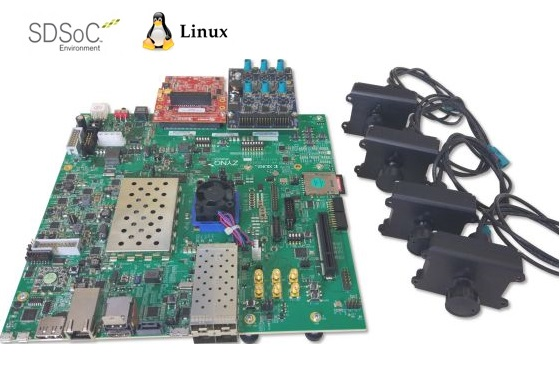
\includegraphics[width=\linewidth]{logiVID-ZU560X.jpg}
    \caption{LogicBricks 4cam system parts \cite{logi_4cam_img}}
    \label{fig:logic_4cam}
\end{figure}

\subsection{Avnet Mipi} % 725 characters
There was another similar device at hand.
The AES-FMC-MULTICAM4-G (\cref{fig:avnet_mipi}), by the previously mentioned Avnet\texttrademark company.
This is also an FMC connected 4 sensor camera system.
All sensor consisted of a MAX96705 16-Bit GMSL (Gigabit Multimedia Serial Link) Serializer and an AR0231AT CMOS digital image sensor with an active pixel array of 1928Hx1208V capable of 4-exposure HDR at 30fps.
This is a smaller sensor than the OV10635 but on the other hand, it can do a better resolution, while not sacrifices the HDR capability.
The lack of cover and the modular assembly, however, makes it more vulnerable.
This system uses an open MIPI CSI-2 serial interface.
Although this system has an example project, the project not used specialized IP blocks.
That way self-made designs are easier with this setting.
This makes the integration of the camera module to the other parts easier.
\begin{figure}
    \centering
    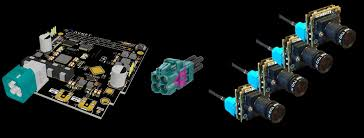
\includegraphics[width=\linewidth]{images/avnet_mipi.jpeg}
    \caption{Avnet 4cam boundle \cite{avnet_mipi_img}}
    \label{fig:avnet_mipi}
\end{figure}

\section{Airsim} % 610 characters
The algorithm that is used for the project is based on a simulator image.
This is the Microsofts\texttrademark Aerial Informatics and Robotics Platform \cite{AirSim} (Airsim for sort), based on the Unreal Engine\texttrademark \cite{UnrealE}.
This is an open-source project that creates a close real environment for testing purposes (\cref{fig:airsim_screen}).
The vehicles can be programmed, to follow a certain path and can be also controlled through an API (Application Programming Interface).
The first is especially comes in hand when the collision is simulated.
It is a hard task to finetune two areal vehicles in the air to collide to each other, in a controlled manner.
In the other hand, the simulator aligns the two trajectories to cross each other, and the record is already usable for the system to detect.
\begin{figure}
    \centering
    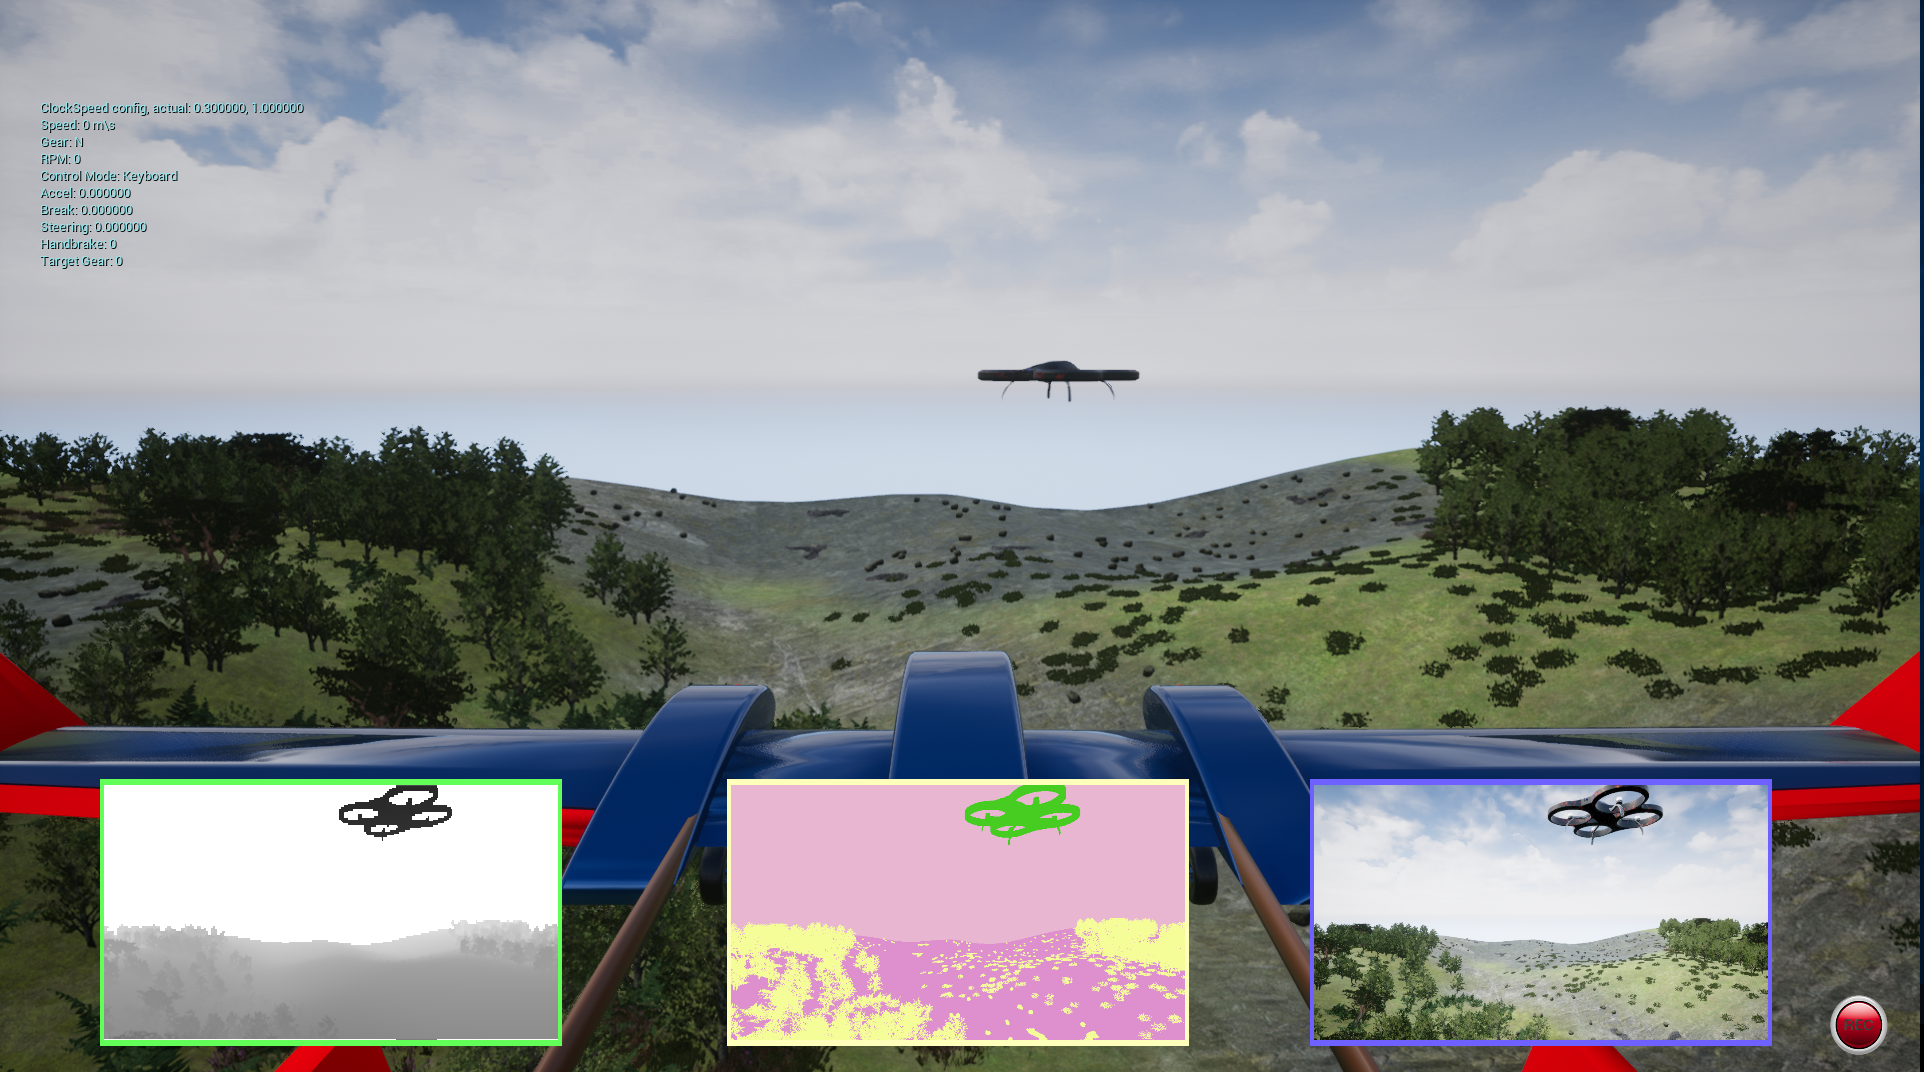
\includegraphics[width=\linewidth]{images/airsim.png}
    \caption{Airsim simulator software screen capture}
    \label{fig:airsim_screen}
\end{figure}

\subsection{HDMI / Ethernet} % 955 characters
There is also a convenient function which is the Ethernet connection.
The API can connect to the simulator through an Ethernet connection using the socket of the program.
This socket can transmit the images from the simulator to the API, which can be processed with the OpenCV (Open source Computer Vision) functions.
This API has a Python and a C++ implementation as well.

The other option to transfer the image to the computing system is through HDMI connection.
The Airsim uses GPU of the simulator server, thus the output video can be redirected to the SoC instead of a display.
For this, there are two possibilities.
The first is the previously mentioned HDMI FMC card from Avnet\texttrademark.
This solution connects the data source to the FPGA directly, witch allows either direct transfer to the output of the same card or accelerated image processing algorithms to applied, limiting the transfer time even further.
There is also an HDMI I/O (Input/Output) port on the ZCU102 as well.
The board has a transceiver subsystem installed, that transfers the data to the PL (Programmable Logic).
For this transceivers, a special programming IP is required.

\subsection{Real flight test} % 409 characters
In a previous conference paper \cite{8798265} the research group described the available hardware.
There are some details of the UAV.
For the real flight test, a 3DR X8+ \cite{x8} (\cref{fig:drone}) will be used, which can carry 800grams.
The UAV is powered by a four-cell Li-Po battery with 14.8V nominal voltage.
There is a DC-DC converter unit onboard, which generates 12V for the FPGA board, and can power up the cameras.
The UAV uses the popular Pixhawk\texttrademark autopilot, which can be connected to the FPGA board through Mavlink protocol \cite{Fuller2014HardwareDA}.
\begin{figure}
    \centering
    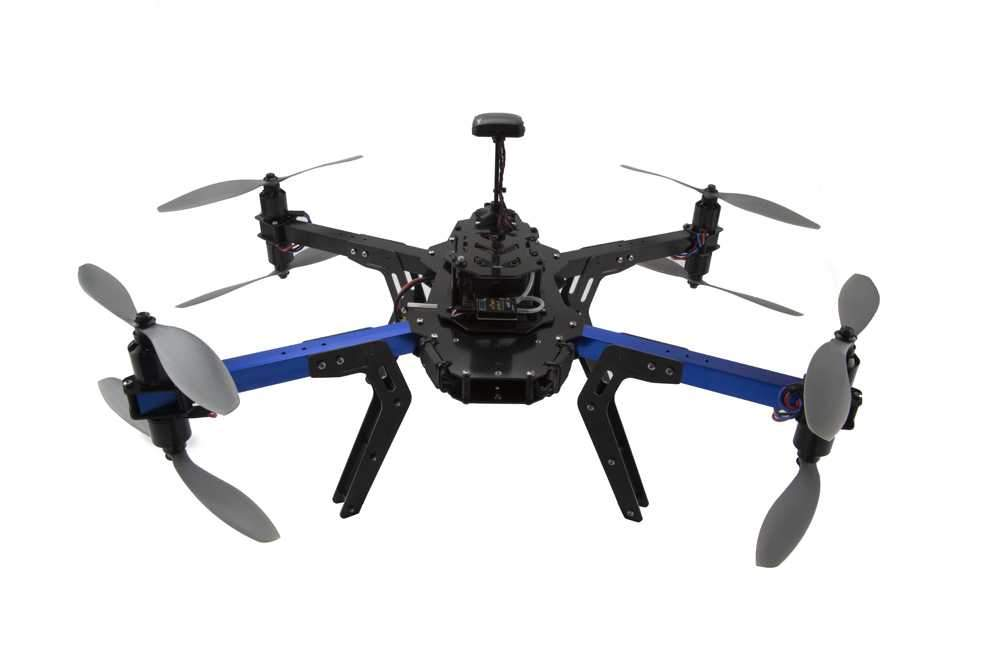
\includegraphics[width=\linewidth]{images/3DR-X8.jpg}
    \caption{The 3DR X8+ drone}
    \label{fig:drone}
\end{figure}

\section{Operating system} % 334 characters
For an embedded system like this, an operating system is required.
Not only the FPGA not working on its own, hence it requires some control unit, but the multiple parts of the whole system require some kind of communication, and execution order.
The PL part could be easily driven by a handmade software, but the loading of the video signals and the other systems requires some higher functionalities.

\subsection{Free Real-Time Operating System} % 955 characters
This operating system is a real-time operating system kernel for embedded devices \cite{FreeROTS}.
The project runs under an MIT (Massachusetts Institute of Technology) free software license.
It is designed to be small and fast.
By limiting the kernel to only 3 files, restricting the allocation policies to strict rules and using multiple threads, the FreeRTOS\texttrademark ensures real-time execution.
This means that by executing a program deterministically, it ensures that the response for an event will be handled in a certain amount of time.
The IoT (Internet of Things) devices and microcontrollers, which are used in automotive systems are required to be deterministic, in order to provide sufficient reaction to the actuators.
In this scenario, the camera input and the control of the drone are both preferred to be deterministic.
Through this OS the drone control can be even transferred to the SoC which saves a computational unit and eliminates one communication connection.

The OS has however little to no support libraries, which makes hard to connect to other systems.
There are also no driver packages which makes hard to connect to the peripheries.

\subsection{Robot Operating System} % 938 characters
The Robot Operating System\texttrademark \cite{ROS} is a Linux Ubuntu\texttrademark based software package, optimised for robotics use.
The OS is modular, and be optimised for low-level device control, hardware abstraction and messaging between subsystems.
It is really good for connecting computer clusters, and embedded devices.
The node like computational graph tough not an RTOS itself provides low latency reactivity.
There are support packages for C++, Python, platform-independent tools and client libraries.
The Airsim environment is also one of the supported packages of the latest ROS.
With this OS the control of the drone could be done as well, even if the original driver unit is not transferred to the SoC, through the communication interface.

The negative side is that the OS is required to run on a full-fledged Ubuntu\texttrademark with all the programs not required by the SoC.
Building the image for a custom hardware architecture, such as the ZCU102 is not as trivial as it seems at first.
The unnecessary parts of the OS, like the simulator environment, also takes up space, and requires resources that are not good for the final product.

\subsection{PetaLinux} % 595 characters
Petalinux\texttrademark is a toolset developed by Xilinx\texttrademark to build embedded Linux systems on the Xilinx\texttrademark processing systems.
In contrast to the previous two, it has drivers, prepared for the Xilinx\texttrademark MPSoCs (MultiProcessor System-on-Chip), and a command-line interface. 
It also includes GCC compiler tools for debugging and system image-building purposes.
The image builder is designed to prepare the BSP (Board Support Package) with only the necessary drivers and libraries.
Through the tools, the Linux kernel can also be altered to the proper purposes.
Asymmetric Multi-Processing (AMP), the possibility to run different tasks on each processing core, is also available, as well as a real-time approach and Xenomai\texttrademark \cite{Xenomai}.

\subsection{PYNQ - Python productivity for Zynq} % 1427 characters
Thy PYNQ \cite{pynq} system is a Python-based development environment for Zynq-7000 SoCs and MPSoCs.
This open-source project is making embedded design easier for high-level programming.
On the processor, a basic PetaLinux\texttrademark and a Jupyter\texttrademark \cite{jupyter} notebook server are running.
This allows the developer to write the algorithm in Python, and run it on the processor, and later accelerate it with the PL part.
The acceleration is done by so-called Overlays.
These overlays are IPs blocks that designed to accelerate time-critical functions of the system and runs on the FPGA part.
Such an overlay is usually developed using VHDL but the software that controls the device can be implemented in Python instead of a standalone C++ application.
The PYNQ system also provides prebuilt overlays, that has an already implemented interface, hence on the Python side, only the function call is required.
On the platform, there is a lot of community-driven projects, of different overlays, such as xfOpenCV which implements OpenCV \cite{xfOpenCV_pynq} functions on PL, or the BNN \cite{finn} which is a framework for a neural network using only binary weights and still performing in a small margin of error, and lot more \cite{rybalkin2017hardware}.

The negative side of the system that is not supported on every board.
On the supported platforms, the usage is easy, but on not supported systems the OS and the overlays must be build from source.
The already built IPs has drivers, the PYNQ system recognises these, and allows access to them through simple function calls.
There is the possibility to design other IPs, but those are not always work properly, and had to program them manually.
This requires the user to write the python wrapper functions, that are already done for the prebuilt overlays.

\section{FPGA development}
% Developing to a hardware platform requires special tools.

\subsection{High-level synthesis} % 503 characters
The HLS (High-level synthesis) is an automated design process to generate hardware systems.
The user has to describe the algorithmic description of the required system in a high-level programming language.
This serially executed code is converted to the parallel executable hardware description, through directives.
The software than transferred to an RTL (Register-Transfer Level) description.
This includes the routing and the required Electric parts, as well as the timing and clocking.
For Xilinx\texttrademark products, the Vivado HLS\texttrademark also creates drivers for the generated IP block for easier integration.

\subsection{Vivado} % 1072 characters
The two main manufacturers of FPGA is Altera\texttrademark and Xilinx\texttrademark.
The University chose to contract with Xilinx\texttrademark that has a slightly more market share.
The Xilinx\texttrademark FPGAs are shipped with the corresponding software and developer tools.
To program these devices, either a hardware description language or prebuilt building blocks must be used.
The Vivado Design Suite\texttrademark is a complex developer software, that allows the users to use either VHDL (VHSIC-HDL) (Very High Speed Integrated Circuit Hardware Description Language) or Verilog languages, to design their software.
Verilog is closer to the hardware level, VHDL allows more abstractions.
Both are usefull to create functionalities.
These code blocks can be imported to block design.
This graphical programming interface allows the users to wire the already working blocks together for more complexity.
In the block design, there also can be included the prebuilt and optimised IP blocks of common applications, like memory access, interconnections, clock generators or the processor subsystem for the SoC devices.
There can be developed also testing circuits, which generates signals and can simulate the working circuit.
This step helps the developer to avoid bugs or even dangerous commands in the hardware design.
The simulation also speeds up the development, since there is no need to programme the device every time, can be done offline and allows detailed examination for the signal changes.
The synthesis can be run if everything works properly.
The synthesis compiles the hardware description and creates a theoretical circuit.
This circuit thus uses the building block included in the FPGA but generates a generally implementable system.
To became device-specific, the synthesised circuit must be implemented on the selected part.
This circuit describes the exact wires and gates the program will use.
The implementation cannot be transferred between devices as the synthesis.
Finally, the implemented circuit should be written to a bitstream file.
This bitstream is the configuration file for the programmable interconnect and the CLBs.
This is a binary file that can be loaded to the device.
The programmed device can be also monitored through USB (Universal Serial Bus) connection with the Vivado\texttrademark.
If the design includes chip scope debug signals, these signal also can be followed by the Vivado\texttrademark debugger waveform display.
Some bitstream requires the processor subsystem to provide a software extension.
For this, the SDK (Software Development Kit) is used where the C++ code can be written and program the hardware as well as the processor.
Amongst the SDK setting can be also set the base OS, program is designed, and the software source will be copiled to that. 
This can be one of the previously mentioned PetaLinux\texttrademark solution, a custom operating system or a standalone application.

\subsection{Software Defined System-on-Chip} % 614 characters
The SDSoC\texttrademark (Software Defined System-on-Chip) is a Xilinx\texttrademark developer program that combines the HLS and the HDL steps.
The algorithm is written in a high level (C++) language and the program creates the IP blocks according to the directives given in the code automatically.
There also preprocessor branchings that separated the hardware implementation from the software.
This marks for the automated workflow, which part should be simulated in the Vivado\texttrademark project, and which will be the basis of the driver.
The resulting system can be transferred to an SD card and be run on the SoC.
This workflow is easier for a fast and small project but it takes the freedom of creating the hardware part.
It also makes it harder to integrate such a system.

\clearpage